\documentclass[12pt]{ufrslides}
\usepackage{textcomp}

\title[CVMFS]{CVMFS}
\author{Helena Rasche}
\date{2018-04-11}

\begin{document}
\frame{\titlepage}

\section{CVMFS}
\begin{frame}{Background}
	\begin{quote}
	The CernVM-File System (CernVM-FS) provides a scalable, reliable and low- maintenance software distribution service
	\end{quote}

	\begin{itemize}
		\item But not just software distribution!
		\item Galaxy Project uses it for worldwide distribution of 6TB of reference data.
	\end{itemize}
\end{frame}

\subsection{Overview}
\begin{frame}{Overview}
	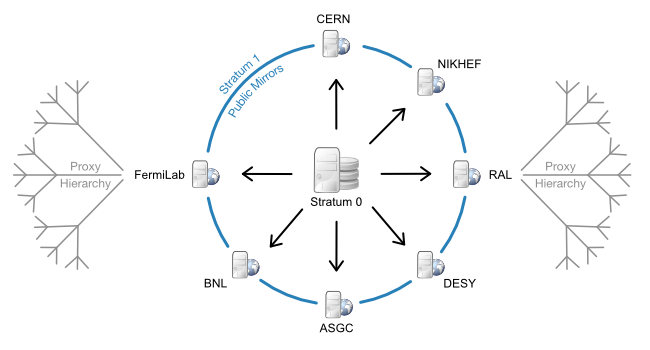
\includegraphics[width=\textwidth]{stratum1.png}
\end{frame}

\begin{frame}{Overview: Path to Data}
	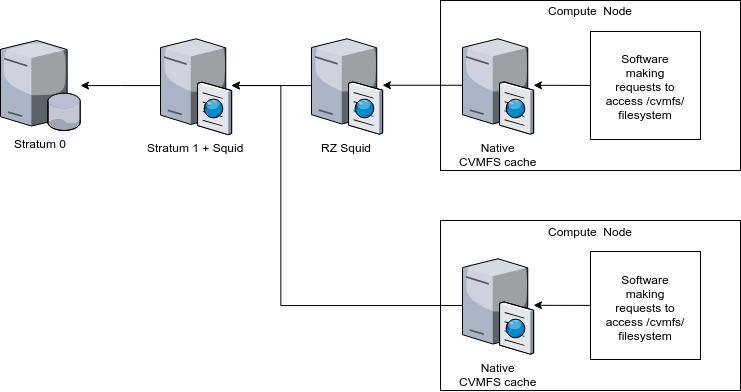
\includegraphics[width=\textwidth]{caching.png}
\end{frame}

\subsection{Internals}
\begin{frame}{Internals}
	\begin{itemize}
		\item Content-addressable storage and Merkle trees for data storage
		\item Outgoing HTTP connections only
		\item On demand transfer of data
		\item Cryptographic hash verification of transfers
	\end{itemize}
\end{frame}

\subsection{Tooling}
\begin{frame}{Standard Tooling}
	\begin{itemize}
		\item Plain HTTP
		\item Standard debugging tools (e.g.~tcpdump, mitmproxy)
		\item Standard HTTP Squid Cache as proxy
		\item Standard caching configuration options (e.g.~size, lifetime, max object size)
		\item Could use CDN services to cache (e.g.~cloudflare, etc.)
	\end{itemize}
\end{frame}

\subsection{Client}
\begin{frame}{Client Viewpoint}
	\begin{itemize}
		\item Read-only filesystem, do not have to care about access control
		\item (Optionally) public distribution network, no secret keys needed (Galaxy Project's is public)
		\item Only up-to-date data
		\item POSIX filesystem via FUSE
		\item Other options if fuse is not available.
	\end{itemize}
\end{frame}

\subsection{Galaxy}
\begin{frame}{Galaxy Project Use}
	\begin{itemize}
		\item \~6TB of reference data
		\item Host multiple stratum1s, one per datacenter
		\item Multiple community hosted stratum1s
		\item Jobs running in VMs leverage ephemeral storage for cvmfs cache
		\item Used in production for the largest known Galaxy server
	\end{itemize}
\end{frame}

\section{Comparison}
\subsection{Rsync}
\begin{frame}{Rsync}
	\begin{itemize}
		\item ``By the aid of the CernVM-FS file catalogs, the \texttt{cvmfs\_server} utility knows beforehand (without remote listing) which files to transfer.''
		\item Easily host only the data your users use
		\item Do not have to know what that is ahead of time
	\end{itemize}
\end{frame}

\subsection{Torrents}
\begin{frame}{Torrents}
	\begin{itemize}
		\item Does not experience firewall issues, university admins often block torrent protocols
		\item Built-in catalog updating, stratum0 pushes a new catalog and everyone automatically updates
		\item (again) Easily host only the data your users use
		\item (again) Do not have to know what that is ahead of time
	\end{itemize}
\end{frame}

\section{Overview}
\begin{frame}{CVMFS Overview}
	\begin{itemize}
		\item Existing example in production with genomics data
		\item Plain HTTP, tons of existing tools
		\item Low client storage requirements, host only want you use
		\item Easy to deploy (ansible roles)
	\end{itemize}
\end{frame}

\end{document}
